\documentclass[tikz]{standalone}

\usepackage{amsmath}
\usetikzlibrary{arrows.meta, positioning}

\tikzstyle{block} = [draw, rectangle, minimum height=3em, minimum width=7em]
\tikzstyle{sum} = [draw, circle]

\begin{document}

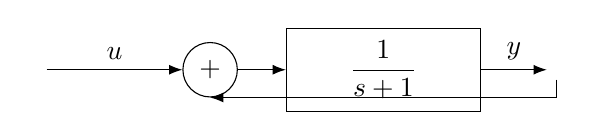
\begin{tikzpicture}[auto, node distance=2.2cm, >=Latex]

\node (input) {};
\node [sum, right of=input] (sum) {$+$};
\node [block, right of=sum] (G) {$\dfrac{1}{s+1}$};
\node (output) [right of=G] {};

\draw [->] (input) -- node {$u$} (sum);
\draw [->] (sum) -- (G);
\draw [->] (G) -- node {$y$} (output);
\draw [->] (output.south) |- (sum.south);

\end{tikzpicture}

\end{document}
